\documentclass[11pt]{article}

\usepackage[margin=1.1in]{geometry}
\usepackage{amsmath,amssymb,amsthm}
\usepackage{mathtools}
\usepackage{booktabs}
\usepackage{tikz}
\usetikzlibrary{arrows.meta,positioning,fit,backgrounds}
\usepackage{xcolor}
\usepackage{enumitem}
\usepackage[colorlinks=true,linkcolor=blue!60!black,citecolor=blue!60!black,urlcolor=blue!60!black]{hyperref}
\usepackage{microtype}

\newtheorem{theorem}{Theorem}[section]
\newtheorem{lemma}[theorem]{Lemma}
\newtheorem{definition}[theorem]{Definition}
\newtheorem{claim}[theorem]{Claim}
\newtheorem{remark}[theorem]{Remark}
\newtheorem*{finding}{Finding}

% ---------- notation (matching sal-mrdts.tex) ----------
\newcommand{\vis}{\xrightarrow{\mathsf{vis}}}
\newcommand{\rc}{\xrightarrow{\mathsf{rc}}}
\newcommand{\rcrel}{\mathsf{rc}}
\newcommand{\comm}{\rightleftarrows}
\newcommand{\ncomm}{\not\rightleftarrows}
\newcommand{\add}{\mathsf{add}}
\newcommand{\rem}{\mathsf{rem}}
\newcommand{\Merge}{\mathsf{merge}}
\newcommand{\mergeL}{\mathsf{merge}}
\newcommand{\Sinit}{\sigma_0}
\newcommand{\loE}[1]{\mathsf{lo}^{#1}}
\newcommand{\lom}{\mathsf{lo}_m}
\newcommand{\lopaper}{\mathsf{lo}}
\newcommand{\dow}[1]{{\downarrow}#1}
\newcommand{\cd}{\mathsf{CDVC3}}
\newcommand{\lean}[1]{\texttt{#1}}
\newcommand{\M}[1]{\mathcal{#1}}
\newcommand{\live}{\mathsf{live}}
% defeater events
\newcommand{\Ap}{A_p}
\newcommand{\Aq}{A_q}
\newcommand{\Rp}{R_p}
\newcommand{\Rq}{R_q}

% ---------- shared TikZ styles (the repo's vtx/stbox family) ----------
\tikzset{
  vtx/.style    ={draw, circle, minimum size=7.5mm, inner sep=0pt,
                  fill=blue!8, line width=0.6pt},
  anc/.style    ={-{Stealth[length=2.2mm]}, line width=0.8pt},
  wit/.style    ={-{Stealth[length=2.2mm]}, line width=1.0pt,
                  red!75!black, densely dashed},
  elbl/.style   ={font=\scriptsize, text=black!60},
  capt/.style   ={font=\small\itshape, text=black!75},
  stbox/.style  ={draw, rounded corners=2pt, inner sep=3.5pt,
                  font=\small, fill=blue!4, line width=0.6pt},
  okbox/.style  ={draw, rounded corners=2pt, inner sep=3.5pt,
                  font=\small, fill=green!7, line width=0.6pt},
  badbox/.style ={draw, rounded corners=2pt, inner sep=3.5pt,
                  font=\small, fill=orange!12, line width=0.6pt},
  lab/.style    ={font=\scriptsize, text=black!65},
}

\title{\bfseries The Defeater, Rule by Rule:\\
\large why the published MRDT soundness proof cannot linearize one
fully LCA-legal merge}
\author{Sal / FP Launchpad (KC + Claude)}
\date{July 18, 2026}

\begin{document}
\maketitle
\sloppy

\begin{abstract}
\noindent
The consolidated Sal note (\texttt{sal-mrdts.pdf}, Part~I) states that a
fully LCA-legal execution defeats the soundness proof of the published
MRDT metatheory, and compresses the argument into one example and one
paragraph. This document decompresses it. We restate the published
proof slowly (the induction, the six-set partition of a merge, and the
eight-law toolbox it consumes), walk the defeater execution version by
version with every state computed and every LCA checked, and then, at
the critical merge, enumerate every move the published toolbox offers:
each of the five merge rules in each orientation, the automation
catalogue behind them, and the natural repairs of the peel architecture
(closure-strengthened peels, block peels, widened induction classes).
Each move fails for a stated, checked reason; every failure is anchored
either to a computation displayed on the page or to a named
kernel-checked theorem
(\lean{no\_inter\_lca\_2op\_rem\_peel\_of\_defeater},
\lean{crack1\_witness}, \lean{reunification\_peel\_obstruction},
\lean{no\_proper\_back\_block}, \lean{killTest\_no\_common\_U}). We then
state precisely what is and is not defeated: the published
\emph{theorem} survives on this execution (the merged version has a
witness, exhibited), the published \emph{proof} does not, and neither
does any peel-shaped repair of it. Finally we run the corrected
metatheory on the very same merge and display the five-line derivation
that discharges it, so the contrast between exhaustion and construction
is visible on one page.
\end{abstract}

\tableofcontents

\paragraph*{Provenance.} The account of the published proof below
follows the paper's own sources: the text of \emph{Automatically
Verifying Replication-aware Linearizability} (the Neem paper) and its
F\textsuperscript{*} artifact interface \lean{App\_mrdt.fsti}, both
vendored in this repository under \lean{\_references/}; no statement
about the published system is reconstructed from memory. The defeater
and every claimed failure are taken from the Lean sources cited inline
(all kernel-checked, zero \lean{sorry}s in the cited chains); where this
document and any compressed prose account could disagree, the Lean is
the ground truth. The general corrected theory is in
\texttt{sal-mrdts.pdf}, Part~I; this document expands its
\S\,``Three facts the metatheory must respect'' and does not replace it.

%======================================================================
\section{What the published proof does}
\label{sec:published}

\subsection{The statement and the induction}

An MRDT is a tuple $\M{D} = \langle \Sigma, \Sinit, \mathsf{do},
\mergeL, \rcrel \rangle$: states $\Sigma$ with initial state $\Sinit$;
$\mathsf{do}$ applies an event $e = (t, r, o)$ (globally unique
timestamp $t$, origin replica $r$, operation $o$), written $e(\sigma)$;
a three-way merge $\mergeL(l, a, b)$ whose first argument is the state
at the lowest common ancestor (LCA) of the two versions being merged;
and a conflict-resolution relation $\rcrel$ that orders concurrent
non-commuting operations. Executions form a version DAG: replicas fork,
apply events, and merge; a version $v$ carries a state $\sigma_v$ and
the set $L(v)$ of events that produced it; visibility $e_1 \vis e_2$
records that $e_2$'s issuing replica had seen $e_1$ when it issued
$e_2$. Write $e_1 \parallel e_2$ for concurrency (neither sees the
other) and $e_1 \comm e_2$ for commutation
($e_1(e_2(\sigma)) = e_2(e_1(\sigma))$ for all $\sigma$).

\begin{definition}[linearization order, per the paper]
\label{def:lo}
$e_1 \mathrel{\lopaper} e_2$ iff
$\bigl(e_1 \vis e_2 \wedge e_1 \ncomm e_2\bigr)$ or
$\bigl(e_1 \parallel e_2 \wedge e_1 \rc e_2 \wedge
\neg\exists e_3.\ e_2 \vis e_3 \wedge e_2 \ncomm e_3\bigr)$.
A visible non-commuting pair is ordered by visibility; a concurrent
$\rcrel$-resolved pair is ordered by $\rcrel$, unless the losing event
already has a later non-commuting observer (an \emph{absorber})
somewhere in the configuration, in which case the $\rcrel$ edge is
dropped. We write $\loE{E}$ for the set-relative variant whose absorber
clause ranges over a set $E$ only; since an absorber anywhere kills a
$\lopaper$ edge, $\lopaper \subseteq \loE{E}$ for every $E$. The paper
uses $\lopaper$; the set-relative variant enters in
\S\ref{sec:walk}--\S\ref{sec:corrected} and the distinction turns out
to matter.
\end{definition}

\begin{definition}[RA-linearizability]
A sequence $\pi$ \emph{witnesses} a version $v$ when (i) $\pi$
enumerates $L(v)$ without repetition, (ii) $\pi$ extends $\lopaper$
(no later element of $\pi$ is $\lopaper$-before an earlier one), and
(iii) $\pi$ folds from $\Sinit$ to $\sigma_v$. A configuration is
RA-linearizable when every version admits a witness.
\end{definition}

The published soundness proof (the paper's Theorem~1, automated as its
Theorem~2) runs an induction on the length of the execution:

\begin{itemize}[leftmargin=2em]
\item \textbf{Assumed at each step}: every version of the current
  configuration is linearizable; in particular each replica head $v$
  has a witness $\pi_v$ that folds to $\sigma_v$.
\item \textbf{Fork} and \textbf{query} change nothing.
  \textbf{Apply} extends a head's witness by the new event:
  $\pi \mapsto \pi e$.
\item \textbf{Merge} is the hard case, and the entire content of the
  proof: given heads $v_1, v_2$ with LCA $v_\top$ (the store guarantees
  $L(v_\top) = L(v_1) \cap L(v_2)$), the new version holds
  $\sigma_m = \mergeL(\sigma_\top, \sigma_1, \sigma_2)$ and event set
  $L(v_1) \cup L(v_2)$, and the proof must \emph{produce} a witness of
  it: a sequence $\pi$ enumerating $L(v_1) \cup L(v_2)$, extending
  $\lom \coloneqq \lopaper$ restricted to that union, and folding to
  $\sigma_m$.
\end{itemize}

\subsection{The merge case: the six-set partition and bottom-up peeling}
\label{sec:partition}

The proof first fixes the \emph{shape} of the witness it will build.
With $L_1 = L(v_1)$, $L_2 = L(v_2)$, $L_\top = L(v_\top)$, it defines
the local events $L_i' = L_i \setminus L_\top$ and splits them by
whether they must precede an LCA event:
\[
  L_i^b = \{e \in L_i' \mid e \text{ is } \lom\text{-before an LCA
  event, directly or via one local event}\}, \quad
  L_i^a = L_i' \setminus L_i^b,
\]
and splits the LCA events into $L_\top^a$ (those with a local
$\lom$-predecessor) and $L_\top^b$ (the rest). Causal closure of
versions makes every pair in $L_1' \times L_2'$ concurrent. The
witness is then assembled in three segments,
\[
  \pi \;=\; \underbrace{S_1}_{L_\top^b} \;
  \underbrace{S_2}_{L_\top^a \cup L_1^b \cup L_2^b} \;
  \underbrace{S_3}_{L_1^a \cup L_2^a},
\]
and the proof constructs $\pi$ \emph{bottom-up}: it repeatedly
\emph{peels} the current last event through the merge, using one of
three interchange rules, and recurses on the smaller merge instance
that remains. A peel does two things at once. It commits one event $e$
to the current last slot of $\pi$, which is legal only if $e$ is
$\lom$-maximal among the events not yet placed (otherwise $\pi$ stops
extending $\lom$). And it rewrites the merge equation, which is
possible only if the rule's arguments \emph{syntactically factor}: the
side an event is peeled from must literally be a $\mathsf{do}$-image
with the peeled operation outermost. There are no front peels in the
published system; every rule extracts the last event.

\subsection{The toolbox: eight laws}
\label{sec:toolbox}

Table~\ref{tab:toolbox} lists the complete toolbox the published merge
case consumes: three constraint laws on the update layer and five merge
laws, of which three are the peel rules.

\begin{table}[t]
\centering
\small
\begin{tabular}{@{}lp{5.9cm}p{5.3cm}@{}}
\toprule
Law & Statement (shape) & Role at a merge step \\
\midrule
\textsc{rc-non-comm} &
for distinct events on different replicas: $\rcrel$ returns
$\mathsf{Either}$ iff the pair commutes &
ties the conflict table to the commutation table; arbitration is
exactly where it is needed \\
\textsc{no-rc-chain} &
never $o_1 \rc o_2$ and $o_2 \rc o_3$ &
keeps $\lopaper$ acyclic, so maximal (peelable-last) events exist \\
\textsc{cond-comm} &
after $o_1 \rc o_2$ is applied in either order, any later
non-commuting $o_3$ erases the difference (base + inductive form) &
lets differently-ordered replays agree; the convergence engine \\
\addlinespace
\textsc{MergeCommutativity} &
$\mergeL(l,a,b) = \mergeL(l,b,a)$ &
halves the rule set: every peel exists in both side orientations \\
\textsc{MergeIdempotence} &
$\mergeL(a,a,a) = a$ &
terminates the derivation once only shared events remain \\
\addlinespace
\textsc{BottomUp-2-OP} &
$e_1 \neq e_2$, $e_1 \rc e_2 \vee e_1 \comm e_2$
$\;\Longrightarrow\;
\mergeL(l, e_1(a), e_2(b)) = e_2(\mergeL(l, e_1(a), b))$ &
peels the last local event when \emph{both} sides still hold
unlinearized local events ($L_1^a, L_2^a \neq \emptyset$) \\
\textsc{BottomUp-1-OP} &
$\mergeL(e_\top(l), e_1(a), e_\top(b)) =
e_1(\mergeL(e_\top(l), a, e_\top(b)))$ &
peels the last local event of the one remaining side, under a shared
trailing LCA event ($L_2^a = \emptyset$) \\
\textsc{BottomUp-0-OP} &
$\mergeL(e_\top(l), e_\top(a), e_\top(b)) = e_\top(\mergeL(l, a, b))$ &
peels a shared LCA event, present outermost on \emph{all three}
arguments ($L_1^a = L_2^a = \emptyset$) \\
\bottomrule
\end{tabular}
\caption{The published toolbox: the three update-layer constraints and
the five merge laws of the paper's Theorem~1. The derivation schedule
is: \textsc{2-OP}/\textsc{1-OP} until $S_3$ is exhausted, then
alternating \textsc{0-OP} (for $L_\top^a$ events) and
\textsc{2-OP}/\textsc{1-OP} (for the $L_i^b$ events attached to them)
through $S_2$, then \textsc{MergeIdempotence} for $S_1$.}
\label{tab:toolbox}
\end{table}

Two features of the peel rules deserve emphasis, because the defeater
lives exactly on them.

\begin{itemize}[leftmargin=2em]
\item \textbf{The factorization requirement.} In
  \textsc{BottomUp-2-OP}, the state written $e_2(b)$ is universally
  quantified as a \emph{pattern}: to apply the rule to a concrete merge
  $\mergeL(\sigma_\top, \sigma_1, \sigma_2)$ one must exhibit $b$ with
  $\mathsf{do}(b, e_2) = \sigma_2$. If no such $b$ exists, the rule
  does not apply, whatever its side conditions say. The same holds for
  $e_1(a)$ in \textsc{1-OP} and for all three arguments in
  \textsc{0-OP}.
\item \textbf{The arbitration orientations.} A \textsc{2-OP} peel
  consults $\rcrel$: the peeled $e_2$ must either commute with the
  opposite side's pending event $e_1$ or be its $\rcrel$-winner
  ($e_1 \rc e_2$: the winner is applied last). With
  \textsc{MergeCommutativity} each candidate peel therefore exists in
  two orientations (which head sits in the peelable slot), and an
  exhaustive check must cover both.
\end{itemize}

\subsection{The automation layer}

The paper's Theorem~2 replaces each rule of Table~\ref{tab:toolbox} by
an induction scheme over the six event sets, Skolemizing ``holds on
feasible states'' into base-and-step equations an SMT solver can
discharge. In the F\textsuperscript{*} artifact
(\lean{\_references/neem\_fstar\_repo/code/interface/App\_mrdt.fsti})
this is the familiar per-datatype catalogue: the four update-layer
obligations (\lean{rc\_non\_comm}, \lean{no\_rc\_chain},
\lean{cond\_comm\_base}, \lean{cond\_comm\_ind}), the two global merge
laws (\lean{merge\_comm}, \lean{merge\_idem}), and the
\lean{base\_*}/\lean{ind\_*}/\lean{inter\_*} families for the
\textsc{2-OP} and \textsc{1-OP} rules together with \lean{lem\_0op}.
The catalogue proves the \emph{same} rules, restricted to states
reachable through the event-set structure; it adds no new derivation
move. One member matters below: \lean{inter\_lca\_2op}
(\lean{App\_mrdt.fsti}, lines 137--143), the catalogue's incarnation of
the \textsc{2-OP} peel under one shared LCA event $o_l$; its conclusion
\begin{align*}
  &\mergeL\bigl(\mathsf{do}(l, o_l),\;
    \mathsf{do}(\mathsf{do}(a, o_l), o_1),\;
    \mathsf{do}(\mathsf{do}(b, o_l), o_2)\bigr) \\
  &\qquad\qquad =\;
  \mathsf{do}\bigl(\mergeL(\mathsf{do}(l, o_l),\,
    \mathsf{do}(a, o_l),\,
    \mathsf{do}(\mathsf{do}(b, o_l), o_2)),\; o_1\bigr)
\end{align*}
peels $o_1$, and requires the side it is peeled from to have the
syntactic shape $\mathsf{do}(\mathsf{do}(a, o_l), o_1)$ with $o_1$
outermost: the factorization requirement again, in its exact artifact
form. This is the statement the kernel arbiter of \S\ref{sec:exhaust}
tests against.

%======================================================================
\section{The defeater execution, drawn and walked}
\label{sec:walk}

\subsection{The datatype}

The defeater is stated over a one-key add-wins skeleton with tagged
adds (Lean: \lean{AWSet} in
\lean{Sal/CRDTs/Metatheory/Convergence\_CounterModel.lean}; it is the
kernel of the production OR-set family). Component by component:

\begin{center}
\small
\begin{tabular}{@{}ll@{}}
\toprule
$\Sigma$ & pairs $\sigma = (A, D)$ of timestamp sets: $A$ = tags added,
$D$ = tags dead \\
$\Sinit$ & $(\emptyset, \emptyset)$ \\
$\mathsf{do}$ & $\add_t(A, D) = (A \cup \{t\},\, D)$ \qquad
$\rem(A, D) = (A,\, A \cup D)$ \quad (kills everything it sees) \\
$\mergeL$ & $\mergeL(l, (A_1,D_1), (A_2,D_2)) =
(A_1 \cup A_2,\, D_1 \cup D_2)$ \quad (union; the LCA slot is
ignored) \\
$\rcrel$ & $\rem \rc \add$ (add wins a race; all other pairs
$\mathsf{Either}$) \\
query & the \emph{live set} $\live(\sigma) = A \setminus D$ \\
\bottomrule
\end{tabular}
\end{center}

Commutation: $\add \comm \add$ (both insert into $A$),
$\rem \comm \rem$ ($D \coloneqq A \cup D$ is absorbing), and
$\add \ncomm \rem$: $\rem(\add_t(\sigma))$ has $t$ dead,
$\add_t(\rem(\sigma))$ has $t$ live; the state-dependence of $\rem$ is
what makes the pair non-commuting. \textsc{rc-non-comm} and
\textsc{no-rc-chain} hold ($\rcrel$ orders exactly the non-commuting
pairs, in one direction, and no operation both wins and loses); the
skeleton also satisfies \textsc{cond-comm} and the two global merge
laws. It is a legal MRDT, inside the published theory's class.

\subsection{The execution, step by step}

Three replicas: $p$, $q$, and a \emph{staging} replica $s$ that only
merges. Four events, timestamps $1$ to $4$:
\[
  \Ap = (1, p, \add), \qquad
  \Aq = (2, q, \add), \qquad
  \Rp = (3, p, \rem), \qquad
  \Rq = (4, q, \rem).
\]
Figure~\ref{fig:defeater} shows the version DAG;
Table~\ref{tab:versions} tabulates every version. The steps:

\begin{enumerate}[leftmargin=2.2em]
\item \textbf{Initial.} All replicas at $v_0$: $L(v_0) = \emptyset$,
  $\sigma_{v_0} = (\emptyset, \emptyset)$.
\item \textbf{$p$ adds.} $p$ applies $\Ap$ at $v_0$: version $p_1$,
  $L = \{\Ap\}$, state $(\{1\}, \emptyset)$, live $\{1\}$.
\item \textbf{$q$ adds.} $q$ applies $\Aq$ at $v_0$: version $q_1$,
  $L = \{\Aq\}$, state $(\{2\}, \emptyset)$, live $\{2\}$.
\item \textbf{The staging merge.} Replica $s$ merges $p_1$ and $q_1$.
  Their only common ancestor is $v_0$, so $\mathrm{LCA} = v_0$, and
  $L(v_0) = \emptyset = \{\Ap\} \cap \{\Aq\}$: \emph{LCA-legal}. New
  version $v_s$, $L = \{\Ap, \Aq\}$, state
  $\mergeL((\emptyset,\emptyset), (\{1\},\emptyset), (\{2\},\emptyset))
  = (\{1,2\}, \emptyset)$, live $\{1, 2\}$.
\item \textbf{$p$ removes, having seen only its own add.} $p$ applies
  $\Rp$ at $p_1$ (it has not yet seen $v_s$): version $p_2$,
  $L = \{\Ap, \Rp\}$, state $(\{1\}, \{1\})$, live $\emptyset$.
  Visibility gained: $\Ap \vis \Rp$.
\item \textbf{$q$ removes symmetrically.} $q$ applies $\Rq$ at $q_1$:
  version $q_2$, $L = \{\Aq, \Rq\}$, state $(\{2\}, \{2\})$, live
  $\emptyset$. Visibility: $\Aq \vis \Rq$.
\item \textbf{$p$ merges in the staging version.} $p$ merges $p_2$ and
  $v_s$. Common ancestors: $v_0, p_1$; the LCA is $p_1$, and
  $L(p_1) = \{\Ap\} = \{\Ap,\Rp\} \cap \{\Ap,\Aq\}$: LCA-legal. New
  head $\mathrm{head}_p$, $L = \{\Ap, \Rp, \Aq\}$, state
  $(\{1\},\{1\}) \sqcup (\{1,2\},\emptyset) = (\{1,2\}, \{1\})$,
  \textbf{live $\{2\}$}: $p$'s own tag is dead, the merged-in $\Aq$
  lives.
\item \textbf{$q$ merges in the staging version.} Symmetrically:
  LCA $q_1$, $L(q_1) = \{\Aq\} = \{\Aq,\Rq\} \cap \{\Ap,\Aq\}$,
  LCA-legal. Head $\mathrm{head}_q$, $L = \{\Aq, \Rq, \Ap\}$, state
  $(\{1,2\}, \{2\})$, \textbf{live $\{1\}$}.
\item \textbf{The critical merge.} The two heads merge. Common
  ancestors: $v_0, p_1, q_1, v_s$; all four reach $v_s$
  ($p_1 \to v_s$, $q_1 \to v_s$ are DAG edges), so
  $\mathrm{LCA} = v_s$, uniquely, and
  \[
    L(v_s) = \{\Ap, \Aq\}
    = \{\Ap,\Rp,\Aq\} \cap \{\Aq,\Rq,\Ap\}
    = L(\mathrm{head}_p) \cap L(\mathrm{head}_q):
  \]
  \emph{fully LCA-legal}. The merged version $v_\top$ holds
  $L = \{\Ap, \Rp, \Aq, \Rq\}$ and state
  $(\{1,2\},\{1\}) \sqcup (\{1,2\},\{2\}) = (\{1,2\}, \{1,2\})$:
  \textbf{all dead}.
\end{enumerate}

Nothing about this execution is dishonest or ill-formed: every merge
sits at a unique LCA whose event set is exactly the intersection of the
two sides' histories; timestamps are globally unique; visibility is
exactly program order ($\Ap \vis \Rp$ and $\Aq \vis \Rq$ are the only
edges, since each remove was issued before its replica saw $v_s$). The
staging replica is the one construction the DAG discipline permits that
one might not think of: it \emph{realizes the intersection of two
histories as an honest store version}, and thereby hands the final
merge a fully legal LCA. All nine states are faithful folds, checked in
the kernel (\lean{sp\_eq}, \lean{sq\_eq}, \lean{LCA\_eq},
\lean{head\_p\_eq}, \lean{head\_q\_eq}, \lean{mergedState\_eq},
\lean{head\_p\_live}, \lean{head\_q\_live}, \lean{mergedState\_live} in
\lean{Refutations/InterLca2op\_Defeater\_Arbiter.lean}).

\begin{figure}[t]
\centering
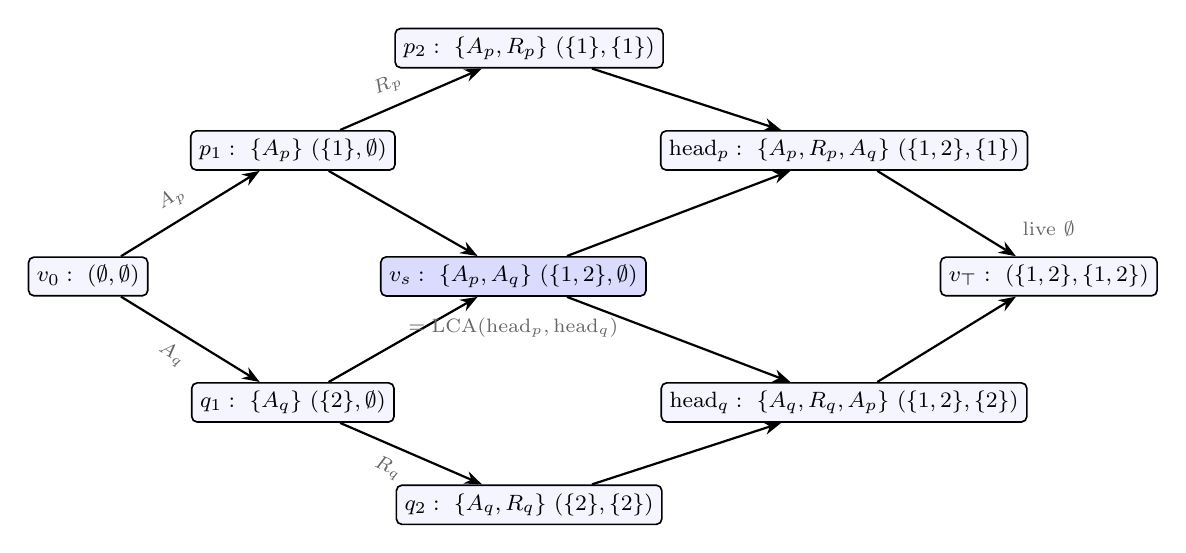
\begin{tikzpicture}[>=Stealth,
  ver/.style={draw, rounded corners=2pt, inner sep=3pt,
    font=\footnotesize, fill=blue!4, line width=0.6pt},
  lca/.style={draw, rounded corners=2pt, inner sep=3pt,
    font=\footnotesize, fill=blue!14, line width=0.6pt},
  lbl/.style={font=\scriptsize, text=black!60}]
\node[ver] (v0) at (0,0) {$v_0:\ (\emptyset,\emptyset)$};
\node[ver] (p1) at (2.6,1.6)  {$p_1:\ \{\Ap\}\ (\{1\},\emptyset)$};
\node[ver] (q1) at (2.6,-1.6) {$q_1:\ \{\Aq\}\ (\{2\},\emptyset)$};
\node[lca] (s)  at (5.4,0)
  {$v_s:\ \{\Ap,\Aq\}\ (\{1,2\},\emptyset)$};
\node[ver] (p2) at (5.6,2.9)  {$p_2:\ \{\Ap,\Rp\}\ (\{1\},\{1\})$};
\node[ver] (q2) at (5.6,-2.9) {$q_2:\ \{\Aq,\Rq\}\ (\{2\},\{2\})$};
\node[ver] (p3) at (9.6,1.6)
  {$\mathrm{head}_p:\ \{\Ap,\Rp,\Aq\}\ (\{1,2\},\{1\})$};
\node[ver] (q3) at (9.6,-1.6)
  {$\mathrm{head}_q:\ \{\Aq,\Rq,\Ap\}\ (\{1,2\},\{2\})$};
\node[ver] (top) at (12.2,0)
  {$v_\top:\ (\{1,2\},\{1,2\})$};
\draw[anc] (v0) -- node[lbl, pos=0.45, above=1pt, sloped]{$\Ap$} (p1);
\draw[anc] (v0) -- node[lbl, pos=0.45, below=1pt, sloped]{$\Aq$} (q1);
\draw[anc] (p1) -- (s);
\draw[anc] (q1) -- (s);
\draw[anc] (p1) -- node[lbl, pos=0.4, above=1pt, sloped]{$\Rp$} (p2);
\draw[anc] (q1) -- node[lbl, pos=0.4, below=1pt, sloped]{$\Rq$} (q2);
\draw[anc] (p2) -- (p3);
\draw[anc] (s)  -- (p3);
\draw[anc] (q2) -- (q3);
\draw[anc] (s)  -- (q3);
\draw[anc] (p3) -- (top);
\draw[anc] (q3) -- (top);
\node[lbl, below=0.14cm of s] {$= \mathrm{LCA}(\mathrm{head}_p,
  \mathrm{head}_q)$};
\node[lbl, above=0.12cm of top] {live $\emptyset$};
\end{tikzpicture}
\caption{The defeater. Versions are labelled with their event sets and
states $(A, D)$; the shaded $v_s$ is the staging version, an honest
store version realizing
$L(\mathrm{head}_p) \cap L(\mathrm{head}_q)$, so the final merge is
fully LCA-legal. Live sets: $\mathrm{head}_p$ lives on $\{2\}$,
$\mathrm{head}_q$ on $\{1\}$, $v_\top$ on nothing.}
\label{fig:defeater}
\end{figure}

\begin{table}[t]
\centering
\footnotesize
\begin{tabular}{@{}llllll@{}}
\toprule
Version & Event set & State $(A,D)$ & Live & Created by & LCA check \\
\midrule
$v_0$ & $\emptyset$ & $(\emptyset,\emptyset)$ & $\emptyset$ & init &
  \\
$p_1$ & $\{\Ap\}$ & $(\{1\},\emptyset)$ & $\{1\}$ & apply $\Ap$ & \\
$q_1$ & $\{\Aq\}$ & $(\{2\},\emptyset)$ & $\{2\}$ & apply $\Aq$ & \\
$v_s$ & $\{\Ap,\Aq\}$ & $(\{1,2\},\emptyset)$ & $\{1,2\}$ &
  merge$(p_1,q_1)$ & $L(v_0)=\emptyset=L(p_1)\cap L(q_1)$ \\
$p_2$ & $\{\Ap,\Rp\}$ & $(\{1\},\{1\})$ & $\emptyset$ & apply $\Rp$ &
  \\
$q_2$ & $\{\Aq,\Rq\}$ & $(\{2\},\{2\})$ & $\emptyset$ & apply $\Rq$ &
  \\
$\mathrm{head}_p$ & $\{\Ap,\Rp,\Aq\}$ & $(\{1,2\},\{1\})$ & $\{2\}$ &
  merge$(p_2,v_s)$ & $L(p_1)=\{\Ap\}=L(p_2)\cap L(v_s)$ \\
$\mathrm{head}_q$ & $\{\Aq,\Rq,\Ap\}$ & $(\{1,2\},\{2\})$ & $\{1\}$ &
  merge$(q_2,v_s)$ & $L(q_1)=\{\Aq\}=L(q_2)\cap L(v_s)$ \\
$v_\top$ & $\{\Ap,\Rp,\Aq,\Rq\}$ & $(\{1,2\},\{1,2\})$ & $\emptyset$ &
  merge$(\mathrm{head}_p,\mathrm{head}_q)$ &
  $L(v_s)=\{\Ap,\Aq\}=$ intersection \\
\bottomrule
\end{tabular}
\caption{Every version of the defeater configuration, with its state
computed and, for each of the four merges, the LCA-legality check.}
\label{tab:versions}
\end{table}

\subsection{The order facts: forced witnesses and the four-event cycle}
\label{sec:orderfacts}

We now compute what witnesses each version admits. The visibility
edges are $\Ap \vis \Rp$ and $\Aq \vis \Rq$; both are non-commuting
pairs, so both are order edges in every variant of the linearization
order. The interesting edges are the $\rcrel$ edges between concurrent
pairs: $\Rp \parallel \Aq$ and $\Rq \parallel \Ap$, both instances of
$\rem \rc \add$. Whether they survive depends on the absorber clause,
and the absorber clause depends on \emph{which event set you look at}:

\begin{itemize}[leftmargin=2em]
\item \textbf{Within $\mathrm{head}_p$'s set
  $E_1 = \{\Ap, \Rp, \Aq\}$}: the candidate absorber for the edge
  $\Rp \to \Aq$ would be a non-commuting vis-successor of $\Aq$ inside
  $E_1$; the only vis-successor of $\Aq$ anywhere is $\Rq$, and
  $\Rq \notin E_1$. The edge \emph{survives}:
  $\Rp \mathrel{\loE{E_1}} \Aq$. Together with $\Ap \to \Rp$ this
  forces the order $[\Ap, \Rp, \Aq]$: the \emph{only}
  $\loE{E_1}$-respecting enumeration of $E_1$.
\item \textbf{Within $\mathrm{head}_q$'s set
  $E_2 = \{\Aq, \Rq, \Ap\}$}: symmetrically, $\Rq \to \Ap$ survives
  ($\Rp \notin E_2$), forcing $[\Aq, \Rq, \Ap]$.
\item \textbf{Within the union $U = \{\Ap, \Rp, \Aq, \Rq\}$}: both
  $\rcrel$ edges are \emph{absorbed}: $\Aq \vis \Rq$ with
  $\Aq \ncomm \Rq$ and $\Rq \in U$ kills $\Rp \to \Aq$; symmetrically
  $\Rp$ kills $\Rq \to \Ap$. So $\lom$ (equivalently $\loE{U}$: on $U$
  the configuration-wide and set-relative orders coincide, because the
  configuration has no events outside $U$) has exactly the two vis
  edges $\Ap \to \Rp$ and $\Aq \to \Rq$. Its maximal events are
  \textbf{$\Rp$ and $\Rq$, and only they}.
\end{itemize}

The state side agrees with the order side, twice over. First, the
forced side orders are also the only \emph{state-correct} ones:
brute-forcing the six enumerations of $E_1$,
\[
\begin{array}{llllll}
[\Ap,\Rp,\Aq] \to (\{1,2\},\{1\})\ \checkmark &
[\Ap,\Aq,\Rp] \to (\{1,2\},\{1,2\}) &
[\Aq,\Ap,\Rp] \to (\{1,2\},\{1,2\}) \\{}
[\Aq,\Rp,\Ap] \to (\{1,2\},\{2\}) &
[\Rp,\Ap,\Aq] \to (\{1,2\},\emptyset) &
[\Rp,\Aq,\Ap] \to (\{1,2\},\emptyset)
\end{array}
\]
only $[\Ap, \Rp, \Aq]$ folds to $\mathrm{head}_p$'s state
$(\{1,2\},\{1\})$: \textbf{every witness of $\mathrm{head}_p$ ends in
$\Aq$}. Symmetrically every witness of $\mathrm{head}_q$ ends in
$\Ap$. Second, at the union: $v_\top$'s state is all-dead, and an
enumeration of $U$ ending in an add folds to a state in which that
add's tag is live (nothing after it can kill it), so \textbf{every
witness of $v_\top$ ends in $\Rp$ or $\Rq$}: exactly the
$\lom$-maximal events, as it must be.

Now glue the two forced side orders (Figure~\ref{fig:cycle}): $E_1$
forces $\Ap < \Rp < \Aq$, $E_2$ forces $\Aq < \Rq < \Ap$. Their union
is the cycle
\[
  \Ap \;\vis\; \Rp \;\xrightarrow{\ \rcrel\ (\text{live in } E_1)\ }\;
  \Aq \;\vis\; \Rq \;\xrightarrow{\ \rcrel\ (\text{live in } E_2)\ }\;
  \Ap .
\]
No total order on $U$ restricts to both side orders. Consequently:

\begin{claim}[the burial]
\label{claim:burial}
No witness of $v_\top$ restricts, on both heads' event sets, to
state-correct witnesses of the heads. Every valid union witness breaks
at least one side: its restriction to that side's event set folds to
the wrong state.
\end{claim}

This is checked in the kernel on a concrete instance:
$w = [\Ap, \Rp, \Aq, \Rq]$ is a valid witness of $v_\top$ (it folds to
the all-dead merged state, \lean{w\_fold}), yet its restriction to
$E_2$ is $[\Ap, \Aq, \Rq]$, which folds to $(\{1,2\},\{1,2\})$ and not
to $\mathrm{head}_q$'s state $(\{1,2\},\{2\})$
(\lean{crack1\_witness}). The events the bottom-up induction must peel
last, the removes, are \emph{buried} mid-history inside the very sides
that own them.

\begin{figure}[t]
\centering
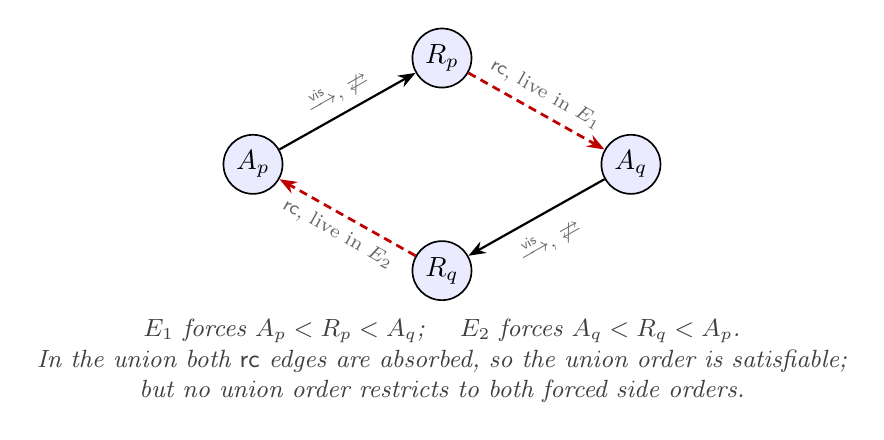
\begin{tikzpicture}[>=Stealth, scale=1.0]
\node[vtx] (ap) at (0,0)    {$\Ap$};
\node[vtx] (rp) at (2.4,1.35)  {$\Rp$};
\node[vtx] (aq) at (4.8,0)  {$\Aq$};
\node[vtx] (rq) at (2.4,-1.35) {$\Rq$};
\draw[anc] (ap) -- node[elbl, above, sloped]
  {$\vis$, $\ncomm$} (rp);
\draw[wit] (rp) -- node[elbl, above, sloped]
  {$\rcrel$, live in $E_1$} (aq);
\draw[anc] (aq) -- node[elbl, below, sloped]
  {$\vis$, $\ncomm$} (rq);
\draw[wit] (rq) -- node[elbl, below, sloped]
  {$\rcrel$, live in $E_2$} (ap);
\node[capt, align=center] at (2.4,-2.5)
  {$E_1$ forces $\Ap < \Rp < \Aq$; \quad $E_2$ forces
   $\Aq < \Rq < \Ap$.\\
   In the union both $\rcrel$ edges are absorbed, so the union order
   is satisfiable;\\
   but no union order restricts to both forced side orders.};
\end{tikzpicture}
\caption{The four-event cycle behind the burial. Solid edges are
visibility edges (present in every event set containing both
endpoints); dashed edges are $\rcrel$ edges, each live only in the side
that lacks its absorber.}
\label{fig:cycle}
\end{figure}

%======================================================================
\section{The critical merge: every move, one by one}
\label{sec:exhaust}

\subsection{What is owed}

At step~9 the induction holds witnesses for $\mathrm{head}_p$,
$\mathrm{head}_q$ (and all earlier versions) and must produce, for the
new version $v_\top$, a sequence $\pi$ such that
\begin{enumerate}[label=(\roman*), leftmargin=2.6em]
\item $\pi$ enumerates $U = \{\Ap, \Rp, \Aq, \Rq\}$ without
  repetition;
\item $\pi$ extends $\lom$, whose edges are exactly $\Ap \to \Rp$ and
  $\Aq \to \Rq$;
\item $\pi$ folds from $\Sinit$ to
  $\sigma_{v_\top} = (\{1,2\}, \{1,2\})$.
\end{enumerate}
The derivation must build $\pi$ back to front by peel steps on the
concrete merge instance
\[
  \mergeL\bigl(\underbrace{(\{1,2\},\emptyset)}_{\sigma_{v_s}},\;
  \underbrace{(\{1,2\},\{1\})}_{\mathrm{head}_p},\;
  \underbrace{(\{1,2\},\{2\})}_{\mathrm{head}_q}\bigr)
  \;=\; (\{1,2\},\{1,2\}).
\]

Before touching the rules, two facts pin down the last slot of $\pi$.
By (ii), the last element must be $\lom$-maximal: $\Rp$ or $\Rq$
(each add has an outgoing $\lom$ edge). By (iii), independently, the
last element must be a remove (a trailing add leaves its tag live,
\S\ref{sec:orderfacts}). So \textbf{every derivation must begin by
peeling a remove}, and the exhaustion below is finite.

One more preliminary, the algebraic heart of everything that follows
(kernel: \lean{awset\_rem\_output\_empty}):

\begin{lemma}[remove images are dead]
\label{lem:remimage}
For every state $s$ and every remove event $e$,
$\live(\mathsf{do}(s, e)) = \emptyset$: indeed
$\rem(A, D) = (A, A \cup D)$ and $A \setminus (A \cup D) = \emptyset$.
Hence a state with a nonempty live set is not a
$\mathsf{do}(\cdot,\rem)$-image of \emph{any} state.
\end{lemma}

Both heads have nonempty live sets: $\live(\mathrm{head}_p) = \{2\}$,
$\live(\mathrm{head}_q) = \{1\}$. Now the moves.

\subsection{The paper's own schedule lands on \textsc{2-OP}}

Computing the six-set partition of \S\ref{sec:partition} for this
merge: $L_1' = \{\Rp\}$, $L_2' = \{\Rq\}$; neither remove is
$\lom$-before any LCA event (their $\rcrel$ edges toward the adds are
absorbed in $\lom$), so $L_1^b = L_2^b = \emptyset$, hence
$L_\top^a = \emptyset$, and
\[
  L_1^a = \{\Rp\}, \qquad L_2^a = \{\Rq\}, \qquad
  L_\top^b = \{\Ap, \Aq\}.
\]
Both $L_1^a$ and $L_2^a$ are nonempty, so the proof's schedule
(Table~\ref{tab:toolbox}) prescribes \textsc{BottomUp-2-OP} as the
first move, peeling the $\lom$-maximal event of one of them. We check
it first, then everything else.

\subsection{Move 1: \textsc{BottomUp-2-OP}, peeling $\Rq$ from
$\mathrm{head}_q$}
\label{sec:move1}

Instantiate $e_2 \coloneqq \Rq$, $e_1 \coloneqq \Rp$. The side
condition holds: $\Rp \neq \Rq$ and $\Rp \comm \Rq$ (removes commute).
The conclusion requires writing the third argument as
$e_2(b)$: a state $b$ with $\mathsf{do}(b, \Rq) = \mathrm{head}_q$.
By Lemma~\ref{lem:remimage} every such image has empty live set, and
$\live(\mathrm{head}_q) = \{1\}$. \textbf{No such $b$ exists; the rule
cannot be instantiated.} Kernel:
\lean{no\_rem\_peelable\_from\_defeater\_heads} (second conjunct).

\subsection{Move 2: \textsc{BottomUp-2-OP}, peeling $\Rp$ from
$\mathrm{head}_p$ (the other orientation)}

Apply \textsc{MergeCommutativity} to swap the heads and peel
$e_2 \coloneqq \Rp$ with $e_1 \coloneqq \Rq$. Side condition: holds,
as before. Factorization: a state $b$ with
$\mathsf{do}(b, \Rp) = \mathrm{head}_p$; $\live(\mathrm{head}_p) =
\{2\} \neq \emptyset$. \textbf{No such $b$ exists.} Kernel:
\lean{no\_rem\_peelable\_from\_defeater\_heads} (first conjunct).

\subsection{Move 3: \textsc{BottomUp-2-OP}, peeling an add}
\label{sec:move3}

The heads \emph{do} factor by adds:
\[
  \mathrm{head}_p = \mathsf{do}(p_2, \Aq)
  \quad\text{since } \mathsf{do}((\{1\},\{1\}), \Aq) =
  (\{1,2\},\{1\}), \qquad
  \mathrm{head}_q = \mathsf{do}(q_2, \Ap),
\]
and the side condition holds ($\Aq \comm \Ap$). The rule's
\emph{equation} is even true here: both sides of
\[
  \mergeL(\sigma_{v_s}, \mathsf{do}(p_2,\Aq),
  \mathsf{do}(q_2,\Ap))
  \;=\;
  \mathsf{do}\bigl(\mergeL(\sigma_{v_s}, \mathsf{do}(p_2,\Aq), q_2),
  \Ap\bigr)
\]
evaluate to $(\{1,2\},\{1,2\})$ (left: the merged state; right:
$\mergeL$ gives $(\{1,2\},\{1\}) \sqcup (\{2\},\{2\}) =
(\{1,2\},\{1,2\})$, and $\Ap$ re-inserts tag $1$, already present).
But a peel is not only an equation: it \emph{commits the peeled event
to the last slot of $\pi$}. Peeling $\Ap$ makes $\pi$ end in $\Ap$
while $\Rp$ remains in the prefix, and $\Ap \mathrel{\lom} \Rp$:
condition (ii) fails. Independently, condition (iii) fails: a
$\pi$ ending in an add folds to a live state, not to
$(\{1,2\},\{1,2\})$; the equation above is consistent with this
because the \emph{recursive} obligation it leaves behind,
linearizing $\mergeL(\sigma_{v_s}, \mathrm{head}_p, q_2)$ over the
event multiset $\{\Ap,\Rp,\Aq\} \cup \{\Aq,\Rq\}$, is not a witness
obligation for $U \setminus \{\Ap\}$ at all ($\Ap$ is still inside
$\mathrm{head}_p$; the event sets no longer partition). The paper's
own induction never proposes this move: it peels only $\lom$-maximal
events, and neither add is $\lom$-maximal. \textbf{The only
factorizations that exist peel events that may not be peeled.}

\subsection{Move 4: \textsc{BottomUp-1-OP}}

The rule is licensed when exactly one of $L_1^a, L_2^a$ is empty; here
both are nonempty, so the schedule never reaches it. Read as a bare
equation anyway: its conclusion peels a local event $e_1$ with the
$a$-side factored as $e_1(a)$, under a shared trailing LCA event
$e_\top$ on the LCA slot and the $b$-side. The shared-event shape is
satisfiable ($e_\top = \Ap$: $\sigma_{v_s} =
\mathsf{do}((\{2\},\emptyset), \Ap)$ and $\mathrm{head}_q =
\mathsf{do}(q_2, \Ap)$), but the peeled $e_1$ must be a
$\lom$-maximal event of the remaining side, i.e.\ $\Rp$, and the
factorization $\mathrm{head}_p = \mathsf{do}(a, \Rp)$ is impossible by
Lemma~\ref{lem:remimage}. Peeling $e_1 = \Aq$ instead repeats
Move~3's failure. \textbf{Dead in both instantiations.}

\subsection{Move 5: \textsc{BottomUp-0-OP}}

The rule peels one shared LCA event $e_\top$, present outermost on
\emph{all three} arguments.
\begin{itemize}[leftmargin=2em]
\item $e_\top$ a remove: the LCA slot must factor,
  $\sigma_{v_s} = \mathsf{do}(l, \rem)$; but
  $\live(\sigma_{v_s}) = \{1,2\} \neq \emptyset$, impossible by
  Lemma~\ref{lem:remimage}. (A remove is not even in $L_\top$, so this
  instantiation was doubly unavailable.)
\item $e_\top = \Aq$ (or symmetrically $\Ap$): all three
  factorizations exist,
  $\sigma_{v_s} = \mathsf{do}((\{1\},\emptyset), \Aq)$,
  $\mathrm{head}_p = \mathsf{do}(p_2, \Aq)$,
  $\mathrm{head}_q = \mathsf{do}((\{1\},\{2\}), \Aq)$; the rule
  instantiates. But it commits $\Aq$ to the last slot of $\pi$, and
  $\Aq \mathrel{\lom} \Rq$ with $\Rq$ unplaced: (ii) fails, and (iii)
  fails as in Move~3. The schedule agrees: \textsc{0-OP} is reached
  only once $S_3 = L_1^a \cup L_2^a$ is exhausted, and
  $S_3 = \{\Rp, \Rq\}$ can never be exhausted (Moves~1 and~2).
\end{itemize}
\textbf{Dead in all instantiations.}

\subsection{Move 6: \textsc{MergeIdempotence} and
\textsc{MergeCommutativity}}

\textsc{MergeIdempotence} requires all three arguments equal; here
they are pairwise distinct ($(\{1,2\},\emptyset)$,
$(\{1,2\},\{1\})$, $(\{1,2\},\{2\})$). Not applicable.
\textsc{MergeCommutativity} is not a peel; it only swaps orientations,
and both orientations of every peel were covered above.

\subsection{Move 7: the automation catalogue}
\label{sec:move7}

Theorem~2's catalogue (\S\ref{sec:toolbox}) discharges the same rules
by induction over the event sets; if no instantiation of a rule exists,
no amount of automation of that rule helps. The kernel makes this
concrete for the catalogue's central member. The arbiter file
\lean{Refutations/InterLca2op\_Defeater\_Arbiter.lean} (written as a
neutral referee for a genuine dispute about exactly this point) proves:

\begin{itemize}[leftmargin=2em]
\item \lean{crux\_no\_rem\_peel\_from\_defeater}: in the
  \lean{inter\_lca\_2op} conclusion shape
  $\mergeL(\mathsf{do}(l,o_l),\, \mathsf{do}(\mathsf{do}(a,o_l),o_1),\,
  \mathsf{do}(\mathsf{do}(b,o_l),o_2))$, none of the four assignments
  (peeled slot $o_1$ or context slot $o_2$; matched to
  $\mathrm{head}_p$ or $\mathrm{head}_q$) can place a remove in the
  outermost position of a head: all four are refuted by
  Lemma~\ref{lem:remimage}.
\item \lean{no\_inter\_lca\_2op\_rem\_peel\_of\_defeater}: therefore
  there is \emph{no} instantiation of \lean{inter\_lca\_2op}'s
  conclusion matching the defeater's merge
  $\mergeL(\sigma_{v_s}, \mathrm{head}_p, \mathrm{head}_q)$, in either
  head-to-slot orientation, in which the peeled operation $o_1$ is a
  remove.
\end{itemize}

The remaining catalogue members (\lean{base\_2op},
\lean{ind\_left/right\_2op}, \lean{inter\_left/right(\_base)\_2op},
and the whole \textsc{1-OP}/\textsc{0-OP} families) share the same
$\mathsf{do}$-outermost peel shape, so the same image fact closes them;
the \textsc{1-OP}/\textsc{0-OP} specifics were covered in
Moves~4 and~5.

\subsection{Move 8: fall back on the induction hypothesis directly}

One might hope to bypass the rules: the sides are linearizable by
assumption, so take their witnesses and interleave them into a union
witness. Claim~\ref{claim:burial} closes this: the side witnesses are
\emph{unique} ($[\Ap,\Rp,\Aq]$ and $[\Aq,\Rq,\Ap]$) and no
interleaving of them is even an order (the four-event cycle of
Figure~\ref{fig:cycle}); conversely, every valid union witness
restricts to a state-\emph{incorrect} sequence on at least one side
(kernel: \lean{crack1\_witness}). The induction hypothesis is not too
weak in degree; it is the wrong \emph{kind} of object: witnesses of
the sides are not raw material for a witness of the union.

\subsection{Interim summary}

\begin{finding}
At the defeater's final merge, the last slot of any witness must hold
$\Rp$ or $\Rq$ (by order and by state); every rule of the published
toolbox that could place a remove there requires a head, or the LCA
state, to be a remove-image, and all three states have nonempty live
sets while every remove-image is dead
(Lemma~\ref{lem:remimage}); the only factorizations that exist peel
adds, which are not $\lom$-maximal and fold wrong; and no assembly of
the (unique) side witnesses is an order. Every rule in the published
toolbox has been tried, in every orientation, and each fails for the
stated reason. This, precisely, is what ``the defeater defeats the
soundness proof'' means.
\end{finding}

\subsection{The repairs that keep the peel, and their refutations}
\label{sec:repairs}

The exhaustion above is relative to the published rule set. Three
natural repairs suggest themselves, each keeping the peel-and-recurse
architecture while strengthening what it may assume. All three are
refuted in the kernel. The refutations are stated not on the AWSet
defeater but on a four-event, two-key configuration $K_2$ distilled
from the same cycle motif; we present it first and are explicit below
about what each theorem does and does not cover.

\paragraph{The kill-test configuration $K_2$.} Two keys $x, y$; four
operations $\add_x, \rem_x, \add_y, \rem_y$; state a pair of
per-key flags; same-key $\rem/\add$ do not commute and are
$\rcrel$-ordered ($\rem_k \rc \add_k$, add wins), cross-key operations
commute (Lean: \lean{K2} in
\lean{Refutations/Reunification\_Peel\_Obstruction.lean}; it satisfies
the update-layer VC bundle, \lean{K2\_updateVCs}, so it is inside the
theory's class). Replica $p$ runs $A_y$ then $R_x$ (so $A_y \vis
R_x$); replica $q$ runs $A_x$ then $R_y$; no communication. Take
$U = \{A_y, R_x, A_x, R_y\}$: it is \emph{fully causally closed}
(every vis-predecessor of a member is a member). The $\rcrel$ edge
$R_x \to A_x$ \emph{survives in $\loE{U}$}, because $A_x$'s only
vis-successor $R_y$ is cross-key and commutes with it, so the absorber
clause cannot fire; symmetrically $R_y \to A_y$ survives. The result
is the cycle
\[
  A_y \;\vis\; R_x \;\xrightarrow{\ \loE{U}\ }\; A_x \;\vis\;
  R_y \;\xrightarrow{\ \loE{U}\ }\; A_y
\]
(kernel: \lean{the\_cycle}): the same alternating vis/$\rcrel$ cycle
as Figure~\ref{fig:cycle}, pushed one level deeper. In the AWSet
defeater the two $\rcrel$ edges are live only per-side and absorbed in
the union; in $K_2$ the cross-key commutation defuses the absorbers,
so the cycle survives \emph{in the union order itself}. $K_2$ is the
minimal habitat in which peel-style repairs must operate, and where
they die.

\paragraph{Repair A: strengthen the bookkeeping to full causal
closure.} Store versions really are fully causally closed (the
published proof itself uses this), so one might re-run a peel
induction that maintains full closure of the shrinking event set,
hoping the stronger invariant licenses stronger per-datatype facts. A
closure-preserving peel of $e$ from a fully closed $U$ needs $e$ to be
simultaneously $\loE{U}$-maximal (placeable last) and
\emph{vis}-maximal (removing it must not orphan a vis edge). On
$K_2$'s $U$: the adds fail vis-maximality (each has a program-order
successor) and the removes fail $\loE{U}$-maximality (each has a
surviving $\rcrel$ edge). \textbf{No event of $U$ is peelable}
(kernel: \lean{no\_peelable\_event}), and the packaged form
\begin{center}
\lean{reunification\_peel\_obstruction}
(\lean{Refutations/Reunification\_Peel\_Obstruction.lean})
\end{center}
exhibits the signature, the configuration (transitive, irreflexive
vis), and the nonempty fully closed $U \subseteq C.\mathsf{events}$
with no such event. Any closure-maintaining single-event peel
induction is stuck at this $U$, whatever VCs it carries.

\paragraph{Repair B: peel a block instead of an event.} Perhaps a
\emph{set} of events can be moved to the end of the enumeration
jointly (on the defeater one is tempted by $\{\Rp, \Rq\}$). Two
generic pins (kernel: \lean{diff\_fullClosure\_iff},
\lean{block\_suffix\_no\_exit}): a back-block $B$ preserves full
closure iff $B$ is vis-upward-closed within $U$, and joint
late-placement forces no $\loE{U}$ edge to leave $B$. On $K_2$'s $U$
these two conditions chase each other around the cycle: vis edges
propagate membership by upward closure, surviving $\rcrel$ edges by
exit-freeness, so \emph{any} nonempty candidate block swallows all of
$U$ (kernel: \lean{back\_block\_forces\_all}), and
\begin{center}
\lean{no\_proper\_back\_block}, \lean{no\_proper\_front\_block}
(\lean{Metatheory/JoinLemma3C.lean})
\end{center}
conclude that no proper back-block and, by the direction-agnostic
cycle, no proper front-block exists: block peels make no progress at
any granularity, from either end. (Scope note, for honesty: on the
AWSet defeater's own $U$ the order-level back-block $\{\Rp, \Rq\}$
\emph{does} exist, and indeed $[\Ap, \Aq, \Rp, \Rq]$ is a valid
witness; what kills block peeling \emph{there} is the same
factorization fact as always, Lemma~\ref{lem:remimage}, since a
published-style block peel must still extract the block's operations
through $\mergeL$ from sides that are not remove-images. The $K_2$
theorem is the stronger, architecture-level statement: even the pure
order-and-closure residue of block peeling, with all state content
deleted, fails in general.)

\paragraph{Repair C: widen the induction class.} If no peel preserves
full closure, let the induction traffic in ``fully closed minus what
has already been peeled'' (\lean{AlmostClosed}: $U \setminus S$ with
$S$ upward-closed under $\loE{U}$). The order theory of this class is
healthy (peels exist and stay in the class:
\lean{AlmostClosed.peel}, \lean{almostClosed\_peel\_exists}), but the
induction on a \emph{merge} needs both sides to decompose over one
\emph{common} fully closed $U$, and the Join hypothesis only supplies
sides that are \emph{individually} fully closed. On the kill-test:
$\mathit{ev}_1 = \{A_y, R_x\}$ and $\mathit{ev}_2 = \{A_x, R_y\}$ are
both fully closed, but any common $U$ decomposing both forces
$S_2 = \{A_y, R_x\}$, which the surviving cross-side edge
$R_x \to A_x$ shows is \emph{not} $\loE{U}$-upward-closed:
\begin{center}
\lean{killTest\_no\_common\_U}
(\lean{Refutations/JoinLemma3F\_Of\_AlmostClosed.lean}).
\end{center}
The widened induction cannot be initialized from what a merge
actually gives it. Concurrent $\rcrel$ edges between the two sides'
exclusive events are exactly what closure, of any strength, does not
control.

\paragraph{Scope of the three refutations.} Repairs A--C and their
refutations arose in the corrected theory's own development (the
reunification study for the enable-wins flag, which needs full-closure
hypotheses); they are cited here because they close, in
machine-checked form, the natural ``why not just\ldots'' branches that
keep the peel architecture alive after \S\ref{sec:move1}--%
\ref{sec:move7}. They are proved on $K_2$, not on the AWSet defeater;
the two configurations share the alternating vis/$\rcrel$ cycle that
is the common cause (Figure~\ref{fig:cycle} vs.\ \lean{the\_cycle}),
and $K_2$ is where that cycle penetrates the union order, which is
what a peel must survive. Note also what the refutations do
\emph{not} say: $K_2$ itself is handled by the corrected weak-closure
route (\lean{weak\_peel\_exists}); only closure-\emph{strengthened}
peels die on it.

\begin{table}[t]
\centering
\small
\begin{tabular}{@{}p{4.6cm}p{5.6cm}p{4.3cm}@{}}
\toprule
Move & Why it fails here & Anchor \\
\midrule
\textsc{2-OP} peel $\Rq$ from $\mathrm{head}_q$ &
$\mathrm{head}_q$ has live $\{1\}$; remove-images are dead: no
factorization &
\lean{awset\_rem\_output\_}\allowbreak\lean{empty},
\lean{no\_rem\_peelable\_\ldots}
\\
\textsc{2-OP} peel $\Rp$ from $\mathrm{head}_p$ (swapped) &
same, live $\{2\}$ &
same, first conjunct \\
\textsc{2-OP} peel an add &
factorization exists, but adds are not $\lom$-maximal: witness stops
extending $\lom$, and folds live &
computation, \S\ref{sec:move3} \\
\textsc{1-OP} &
schedule: both $L_i^a$ nonempty; bare equation: peeled local event
must be a remove, no factorization &
Lemma~\ref{lem:remimage} \\
\textsc{0-OP} &
$e_\top$ a remove: LCA slot live $\{1,2\}$, not an image;
$e_\top$ an add: not $\lom$-maximal &
Lemma~\ref{lem:remimage}, \S\ref{sec:move3} \\
\textsc{MergeIdempotence} &
arguments pairwise distinct &
Table~\ref{tab:versions} \\
\textsc{MergeCommutativity} &
not a peel; both orientations covered &
\\
catalogue (\lean{inter\_lca\_2op} etc.) &
same rules, Skolemized; no instantiation with a peeled remove exists,
either orientation &
\lean{no\_inter\_lca\_2op\_}\allowbreak\lean{rem\_peel\_of\_defeater},
\lean{crux\_no\_rem\_}\allowbreak\lean{peel\_\ldots} \\
interleave the side witnesses &
side witnesses unique and mutually cyclic; every union witness breaks
a side &
\lean{crack1\_witness}, Fig.~\ref{fig:cycle} \\
\midrule
repair A: full-closure single peel &
a fully closed $U$ exists with no $\loE{U}$-maximal and vis-maximal
event &
\lean{reunification\_peel\_}\allowbreak\lean{obstruction} \\
repair B: block peel (back/front) &
on the same $U$, every legal block is all of $U$ &
\lean{no\_proper\_back\_block},
\lean{no\_proper\_front\_block} \\
repair C: widened class (common $U$) &
individually closed sides admit no common $U$: not initializable &
\lean{killTest\_no\_common\_U} \\
\bottomrule
\end{tabular}
\caption{The exhaustion, summarized. Rows above the line are on the
defeater itself; rows below are the architecture-level repairs, refuted
on the $K_2$ kill-test (\S\ref{sec:repairs}).}
\label{tab:exhaust}
\end{table}

%======================================================================
\section{What the defeater does and does not defeat}
\label{sec:scope}

Exactness matters here, because ``defeats the soundness proof'' is
easily misread as ``refutes the theorem.'' It does not.

\paragraph{The theorem survives on this execution.} Every version of
the defeater configuration is RA-linearizable. Witnesses, one per
version, each checkable by the folds already computed in
Table~\ref{tab:versions}: $[\,]$ for $v_0$; $[\Ap]$, $[\Aq]$,
$[\Ap,\Aq]$, $[\Ap,\Rp]$, $[\Aq,\Rq]$ for $p_1, q_1, v_s, p_2, q_2$;
$[\Ap,\Rp,\Aq]$ for $\mathrm{head}_p$; $[\Aq,\Rq,\Ap]$ for
$\mathrm{head}_q$; and for the critical $v_\top$ both
$[\Ap,\Aq,\Rp,\Rq]$ and $w = [\Ap,\Rp,\Aq,\Rq]$ fold to
$(\{1,2\},\{1,2\})$ and extend $\lom$ (kernel, for $w$:
\lean{w\_fold}). So the defeater is \emph{not} a counterexample to the
published Theorem~1 or Theorem~2 as statements about this datatype
(the AWSet skeleton in fact satisfies a corrected contract and is
linearizable at every reachable configuration,
\S\ref{sec:corrected}). Whether the published \emph{statement} holds
for every datatype satisfying its VCs is thereby left open by the
defeater alone, refuted for no datatype and proved for none: what is
refuted is the only proof on offer.

\paragraph{What is defeated, precisely.}
\begin{enumerate}[leftmargin=2.2em]
\item \textbf{The derivation.} The bottom-up proof of Theorem~1 must,
  at the merge of step~9, produce a witness using the eight laws;
  \S\ref{sec:exhaust} shows no first move exists. The proof, as
  written, does not establish its theorem. The automation of
  Theorem~2 automates the same rules and inherits the failure
  (\S\ref{sec:move7}).
\item \textbf{The proof's central invariant.} The induction
  manufactures merged witnesses out of \emph{state-correct side
  witnesses}. On the defeater the side witnesses are unique, mutually
  cyclic, and no valid union witness restricts to both
  (Claim~\ref{claim:burial}, \lean{crack1\_witness}): the invariant is
  not just unprovable here, it is false as a description of how the
  union witness relates to the sides.
\item \textbf{The configuration-wide order, as an internal tool.} With
  the paper's $\lopaper$, the restriction to $E_1$ has no edge
  $\Rp \to \Aq$ (the absorber $\Rq$ exists in the configuration), so
  both $[\Ap,\Rp,\Aq]$ and $[\Ap,\Aq,\Rp]$ extend
  $\lopaper|_{E_1}$, yet they fold to different states
  (\S\ref{sec:orderfacts}). Any internal lemma of the form ``all
  order-respecting replays of a version agree'' is false for
  $\lopaper$; the corrected theory's set-relative $\loE{E}$ exists
  precisely to make it true. (RA-linearizability itself only asserts
  existence of a witness, so this is a defect of the proof
  machinery, not of the definition; and since
  $\lopaper \subseteq \loE{E}$, witnesses built against $\loE{E}$
  deliver the paper's definition verbatim.)
\item \textbf{Every peel-shaped repair} that Table~\ref{tab:exhaust}
  lists: closure-strengthened single peels, block peels in both
  directions, and the widened-class initialization, each by a named
  kernel theorem on $K_2$.
\end{enumerate}

Adjacent but distinct: the store-level LCA lemma
($L(v_\ell) = L(v_1) \cap L(v_2)$) is \emph{true} and the defeater
exercises it honestly at all four merges; its published proof has a
separate, orthogonal gap (a missing generator-uniqueness induction),
mechanized and repaired in \lean{Metatheory/LCA\_Lemma.lean} and
discussed in \texttt{sal-mrdts.pdf} \S4.1. Nothing in this document
depends on that gap.

%======================================================================
\section{How the corrected theory handles the same execution}
\label{sec:corrected}

The corrected metatheory (\texttt{sal-mrdts.pdf}, Part~I,
\S5--\S8) draws the architectural conclusion of
Claim~\ref{claim:burial}: witnesses for a merged version cannot be
manufactured out of witnesses for its sides, so the proof must not
traffic in witness lists at all. Its objects are \emph{canonical
states}: the update layer proves (from the three update-layer VCs,
now with the set-relative $\loE{E}$) that all $\loE{E}$-respecting
enumerations of a finite $E$ fold to the same state, written
$\sigma(E)$; the merge layer then owes exactly one equation per merge,
the ternary \emph{Join Lemma}
\[
  \sigma(E_1 \cup E_2) \;=\;
  \mergeL\bigl(\sigma(E_1 \cap E_2),\, \sigma(E_1),\, \sigma(E_2)\bigr),
\]
whose first argument is, by the LCA lemma, exactly the state the store
hands the merge. The per-datatype contract behind it is eight VCs
(\texttt{sal-mrdts.pdf} \S7): the three update-layer laws
(\textsc{rc-non-comm} with a different-replica guard,
\textsc{no-rc-chain}, \textsc{cond-comm}), merge symmetry, and four
merge-layer laws quantified over \emph{canonical} tuples at honest
LCAs: the feasible unit law, two \emph{redistribution} identities
(\textsc{local-redistribute} and \textsc{redistribute}, the delta
contract), and the \emph{causal-delta} equation
\[
  \cd: \qquad
  \mergeL\bigl(B,\; A,\; e(B)\bigr) \;=\; e(A)
\]
for $e$ a $\loE{U}$-maximal event of a backward-closed $U$, with
$A = \sigma(U \setminus \{e\})$ and
$B = \sigma(\dow{e} \setminus \{e\})$ the canonical state of $e$'s own
causal past: ``what an event does is determined by what it saw.'' The master
induction (\lean{join\_lemma3\_of\_cd\_feasible},
\lean{Metatheory/Adequacy.lean}) proves the Join Lemma from these by
strong induction on $|E_1 \cup E_2|$, and the transition induction
(\lean{ra\_linearizable\_of\_core\_feasible\_cd3}) maintains ``every
store version holds $\sigma$ of its event set,'' which is
RA-linearizability per version. We now run that induction on the
defeater's critical merge and watch it construct what
\S\ref{sec:exhaust} proved unreachable.

\subsection{The same merge, discharged in five lines}

The instance: $E_1 = \{\Ap,\Rp,\Aq\}$, $E_2 = \{\Aq,\Rq,\Ap\}$,
$E_1 \cap E_2 = \{\Ap,\Aq\}$, $U = E_1 \cup E_2$ all four events. The
canonical states (all computed in \S\ref{sec:walk}; the unique
respecting enumerations are the forced witnesses):
\[
  s_0 = \sigma(E_1 \cap E_2) = (\{1,2\},\emptyset), \quad
  s_1 = \sigma(E_1) = (\{1,2\},\{1\}), \quad
  s_2 = \sigma(E_2) = (\{1,2\},\{2\}).
\]
Goal: $\mergeL(s_0, s_1, s_2) = \sigma(U) = (\{1,2\},\{1,2\})$.

\textbf{Step 1: select a $\loE{U}$-maximal event}
(\lean{exists\_loOn\_maximal\_u}). The maximal events are $\Rp$ and
$\Rq$ (\S\ref{sec:orderfacts}); take $e = \Rq$. Note what just
happened: the corrected induction picks its pivot by the
\emph{union's} order, where $\Rq$'s $\rcrel$ edge is absorbed; it is
entirely indifferent to the fact that $\Rq$ is buried inside $E_2$'s
own order. Its data:
\[
  \dow{\Rq} = \{\Aq, \Rq\}, \qquad
  B = \sigma(\dow{\Rq} \setminus \{\Rq\}) = \sigma(\{\Aq\}) =
  (\{2\},\emptyset), \qquad
  e(B) = \Rq(B) = (\{2\},\{2\}),
\]
\[
  A = \sigma(U \setminus \{\Rq\}) = \sigma(\{\Ap,\Rp,\Aq\}) =
  (\{1,2\},\{1\}) \quad (= s_1: \text{here } U \setminus \{\Rq\}
  \text{ happens to equal } E_1).
\]

\textbf{Step 2: decompose the side that owns $e$}
(\lean{side\_decompositionF}). Since $\Rq \in E_2$ only, the induction
rewrites $E_2$ as a \emph{join of event sets},
$E_2 = (E_2 \setminus \{\Rq\}) \cup \dow{\Rq}$ with intersection
$\dow{\Rq} \setminus \{\Rq\}$, and applies the induction hypothesis at
this smaller union (three events) to get
\[
  s_2 \;=\; \mergeL\bigl(B,\; t_2,\; \Rq(B)\bigr),
  \qquad t_2 = \sigma(E_2 \setminus \{\Rq\}) = \sigma(\{\Aq,\Ap\}) =
  (\{1,2\},\emptyset).
\]
Numerically: $\mergeL((\{2\},\emptyset), (\{1,2\},\emptyset),
(\{2\},\{2\})) = (\{1,2\},\{2\}) = s_2$. $\checkmark$
This is the move the published system does not have: it does not ask
how $s_2$ \emph{factors through} $\mathsf{do}$ (it does not, by
Lemma~\ref{lem:remimage}); it decomposes $E_2$ \emph{through the
join}, with the merge's own LCA slot ($B$, the state of $\Rq$'s causal
past) doing the bookkeeping. Inside the recursive call, the union
$E_2$ selects \emph{its own} maximal event, which is $\Ap$ (in
$\loE{E_2}$ the edge $\Rq \to \Ap$ is live, so $\Ap$ is last), i.e.\
the recursion peels on that level exactly the event the forced witness
$[\Aq,\Rq,\Ap]$ ends with. Set-relativity is what lets different
levels peel different events.

\textbf{Step 3: redistribute the delta}
(\lean{FeasibleDeltaVCs3.feasible\_local\_redistribute}). Read
$c = \Rq(B)$ as a delta relative to $m = B$. The
\textsc{local-redistribute} law
$\mergeL(l, \mergeL(m, x, c), y) = \mergeL(m, \mergeL(l, x, y), c)$,
instantiated at $l = s_0$, $x = t_2$, $y = s_1$ (using merge symmetry
to place the decomposed side), turns the goal's left side into
\[
  \mergeL(s_0, s_1, s_2)
  = \mergeL\bigl(s_0,\, s_1,\, \mergeL(B, t_2, \Rq(B))\bigr)
  = \mergeL\bigl(B,\; \mergeL(s_0, s_1, t_2),\; \Rq(B)\bigr).
\]

\textbf{Step 4: the inner join, by the induction hypothesis.} The
inner merge is a Join Lemma instance at
$E_1 \cup (E_2 \setminus \{\Rq\}) = U \setminus \{\Rq\}$ with
intersection $E_1 \cap (E_2 \setminus \{\Rq\}) = \{\Ap,\Aq\}$: three
events, strictly smaller, so the IH gives
\[
  \mergeL(s_0, s_1, t_2) = \sigma(U \setminus \{\Rq\}) = A .
\]
Numerically: $\mergeL((\{1,2\},\emptyset), (\{1,2\},\{1\}),
(\{1,2\},\emptyset)) = (\{1,2\},\{1\}) = A$. $\checkmark$

\textbf{Step 5: close with the causal-delta equation and snoc.} The
$\cd$ VC at $U$, $e = \Rq$ (its hypotheses are exactly satisfied:
$U$ backward-closed, $\Rq$ maximal, $A$ and $B$ canonical):
\begin{gather*}
  \mergeL\bigl(B, A, \Rq(B)\bigr) = \Rq(A), \qquad
  \text{numerically:} \\
  \mergeL\bigl((\{2\},\emptyset), (\{1,2\},\{1\}),
  (\{2\},\{2\})\bigr) = (\{1,2\},\{1,2\}) = \Rq((\{1,2\},\{1\})).
  \;\checkmark
\end{gather*}
Finally $\Rq(A) = \sigma(U)$ because $A$ is canonical for
$U \setminus \{\Rq\}$ and $\Rq$ is $\loE{U}$-maximal
(\lean{isCanonicalState\_snoc}): appending a maximal event to a
canonical enumeration is again canonical. Chaining steps 2--5:
\begin{align*}
  \mergeL(s_0, s_1, s_2)
  &\;=\; \mergeL\bigl(B,\, \mergeL(s_0,s_1,t_2),\, \Rq(B)\bigr) \\
  &\;=\; \mergeL\bigl(B,\, A,\, \Rq(B)\bigr)
  \;=\; \Rq(A)
  \;=\; \sigma(U). \qquad \blacksquare
\end{align*}

The witness object this constructs for $v_\top$ is any
$\loE{U}$-respecting enumeration, concretely $[\Ap,\Rp,\Aq]$ (the
canonical enumeration of $A$'s set) followed by $\Rq$: that is,
$w = [\Ap, \Rp, \Aq, \Rq]$, exactly the ``tempting linearization''
that \S\ref{sec:exhaust} could see but never derive. The corrected
proof derives it \emph{without ever claiming} that $w$ restricts to
state-correct side witnesses (it does not: \lean{crack1\_witness});
the sides enter the argument only through their canonical
\emph{states} $s_1, s_2$ and the three merge-layer equations. The
burial pathology has nothing left to grip.

\subsection{Why the $\cd$ instance is true here, and in general}

It is worth seeing why $\cd$ holds at step~5, since it is the one
genuinely per-datatype fact consumed. For the add-wins skeleton,
$\mergeL(B, A, \Rq(B))$ has dead set
$D_A \cup A_B \cup D_B$ while $\Rq(A)$ has dead set $A_A \cup D_A$; the
two agree iff every tag live in $A$ was seen by $\Rq$ (is in $A_B$).
That is false for arbitrary tuples, and true here \emph{because $\Rq$
is $\loE{U}$-maximal}: a concurrent add in $U$ either lies in
$\dow{\Rq}$ (then its tag is in $A_B$), or it has a non-commuting
vis-successor in $U$ that absorbs the $\rcrel$ edge (then it is
already dead in $A$). On the instance: the concurrent $\Ap \notin
\dow{\Rq}$, and indeed $1 \in D_A$, absorbed by $\Rp$. This trichotomy
is the uniform discharge recipe for $\cd$ across the catalogue, and it
is precisely the feasibility conditioning the published catalogue's
$\forall$-quantified VCs lack: the same equation quantified over all
states is false (take $A$ with a live tag $\Rq$ never saw and no
absorber).

\subsection{Where this instance sits in the corrected architecture}

For the record, the route just walked is the weak-closure instance of
the closure-indexed contract: the corrected Join Lemma is stated once
as $\mathsf{JoinLemma3C}\,\mathcal{C}$, indexed by the closure
predicate $\mathcal{C}$ the datatype declares
(\lean{Metatheory/JoinLemma3C.lean}); the add-wins family sits at weak
closure (the hypotheses used in steps 1--5), the enable-wins flag at
full closure, and the soundness bridge
\lean{ra\_linearizable3\_of\_joinC}
(\lean{Metatheory/ConditionedContract.lean}) is uniform across
strengths because store versions are fully closed and full closure
implies every declared $\mathcal{C}$. That index exists \emph{because}
of \S\ref{sec:repairs}: the refutations
\lean{reunification\_peel\_obstruction} /
\lean{no\_proper\_back\_block} / \lean{killTest\_no\_common\_U} show
the two strengths cannot be reunified into one induction, so the
contract carries the index instead of pretending to. The production
OR-set, whose kernel the defeater's skeleton is, is discharged
end-to-end through this architecture
(\lean{ORSet\_ra\_linearizable3\_eq}).

%======================================================================
\section{The lesson, in one paragraph}
\label{sec:lesson}

What the published toolbox could not see is that \emph{being last} is
not a property of an event, nor of a state, but of an event
\emph{relative to an event set}. Every published rule reads finality
off a state factorization: ``the side is
$\mathsf{do}(b, e)$, so $e$ may go last.'' The defeater manufactures,
with one staging replica and full LCA legality, a merge whose sides
are factorizable only by events that must \emph{not} go last (the
adds, absorbed in the union but binding per-side) while the events
that must go last (the removes) are buried mid-history on their own
sides and leave no trace in any factorization of the head states
(remove-images are dead; the heads are live). Finality flips between
$E_1$, $E_2$, and $U$ because the absorber clause is set-relative,
and a toolbox whose every move is surgery on side \emph{witnesses}
cannot follow it. The corrected theory follows it by construction: its
induction is surgery on \emph{histories} (decompose $E_2$ as
$(E_2 \setminus \{e\}) \sqcup \dow{e}$, at the honest LCA
$\dow{e} \setminus \{e\}$), its per-datatype laws are equations
between canonical states of event sets, and the one place finality is
consulted ($\loE{U}$-maximality, feeding $\cd$) names the set it is
relative to.

\paragraph{Pointers.} The general theory this document instantiates:
\texttt{sal-mrdts.pdf}, Part~I: \S3 (the ternary setting and the
set-relative order), \S4.1 (the LCA lemma's separate gap), \S4.2 (the
defeater, compressed), \S5 (canonical states and the Join Lemma), \S6
(why the contract is a delta contract), \S7 (the eight corrected VCs
and the $\cd$ recipe), \S8 (adequacy, the closure-indexed contract,
and the reunification finding), \S9 (the discharged catalogue). The
kernel anchors cited here: \lean{Refutations/}%
\lean{InterLca2op\_Defeater\_Arbiter.lean} (the defeater, its states,
and the peel refutations), \lean{Refutations/}%
\lean{Reunification\_Peel\_Obstruction.lean} (the $K_2$ kill-test),
\lean{Refutations/JoinLemma3F\_Of\_AlmostClosed.lean} (the common-$U$
refutation), \lean{Metatheory/JoinLemma3C.lean} (block peels; the
closure index), \lean{Metatheory/Adequacy.lean} (the corrected master
induction), all kernel-checked with clean axioms.

\end{document}
